\documentclass{article}

\usepackage{graphicx}
\usepackage{tikz}
\usepackage{tikzsymbols}
\usetikzlibrary{calc,patterns,shapes.geometric}
\pagestyle{empty}
\usepackage[margin=0pt]{geometry}
\geometry{papersize={14in,12in}}

\def\centerarc[#1](#2)(#3:#4:#5){\draw[#1] ($(#2)+({#5*cos(#3)},{#5*sin(#3)})$) arc (#3:#4:#5);}

\begin{document}
	\begin{figure}
		\centering
		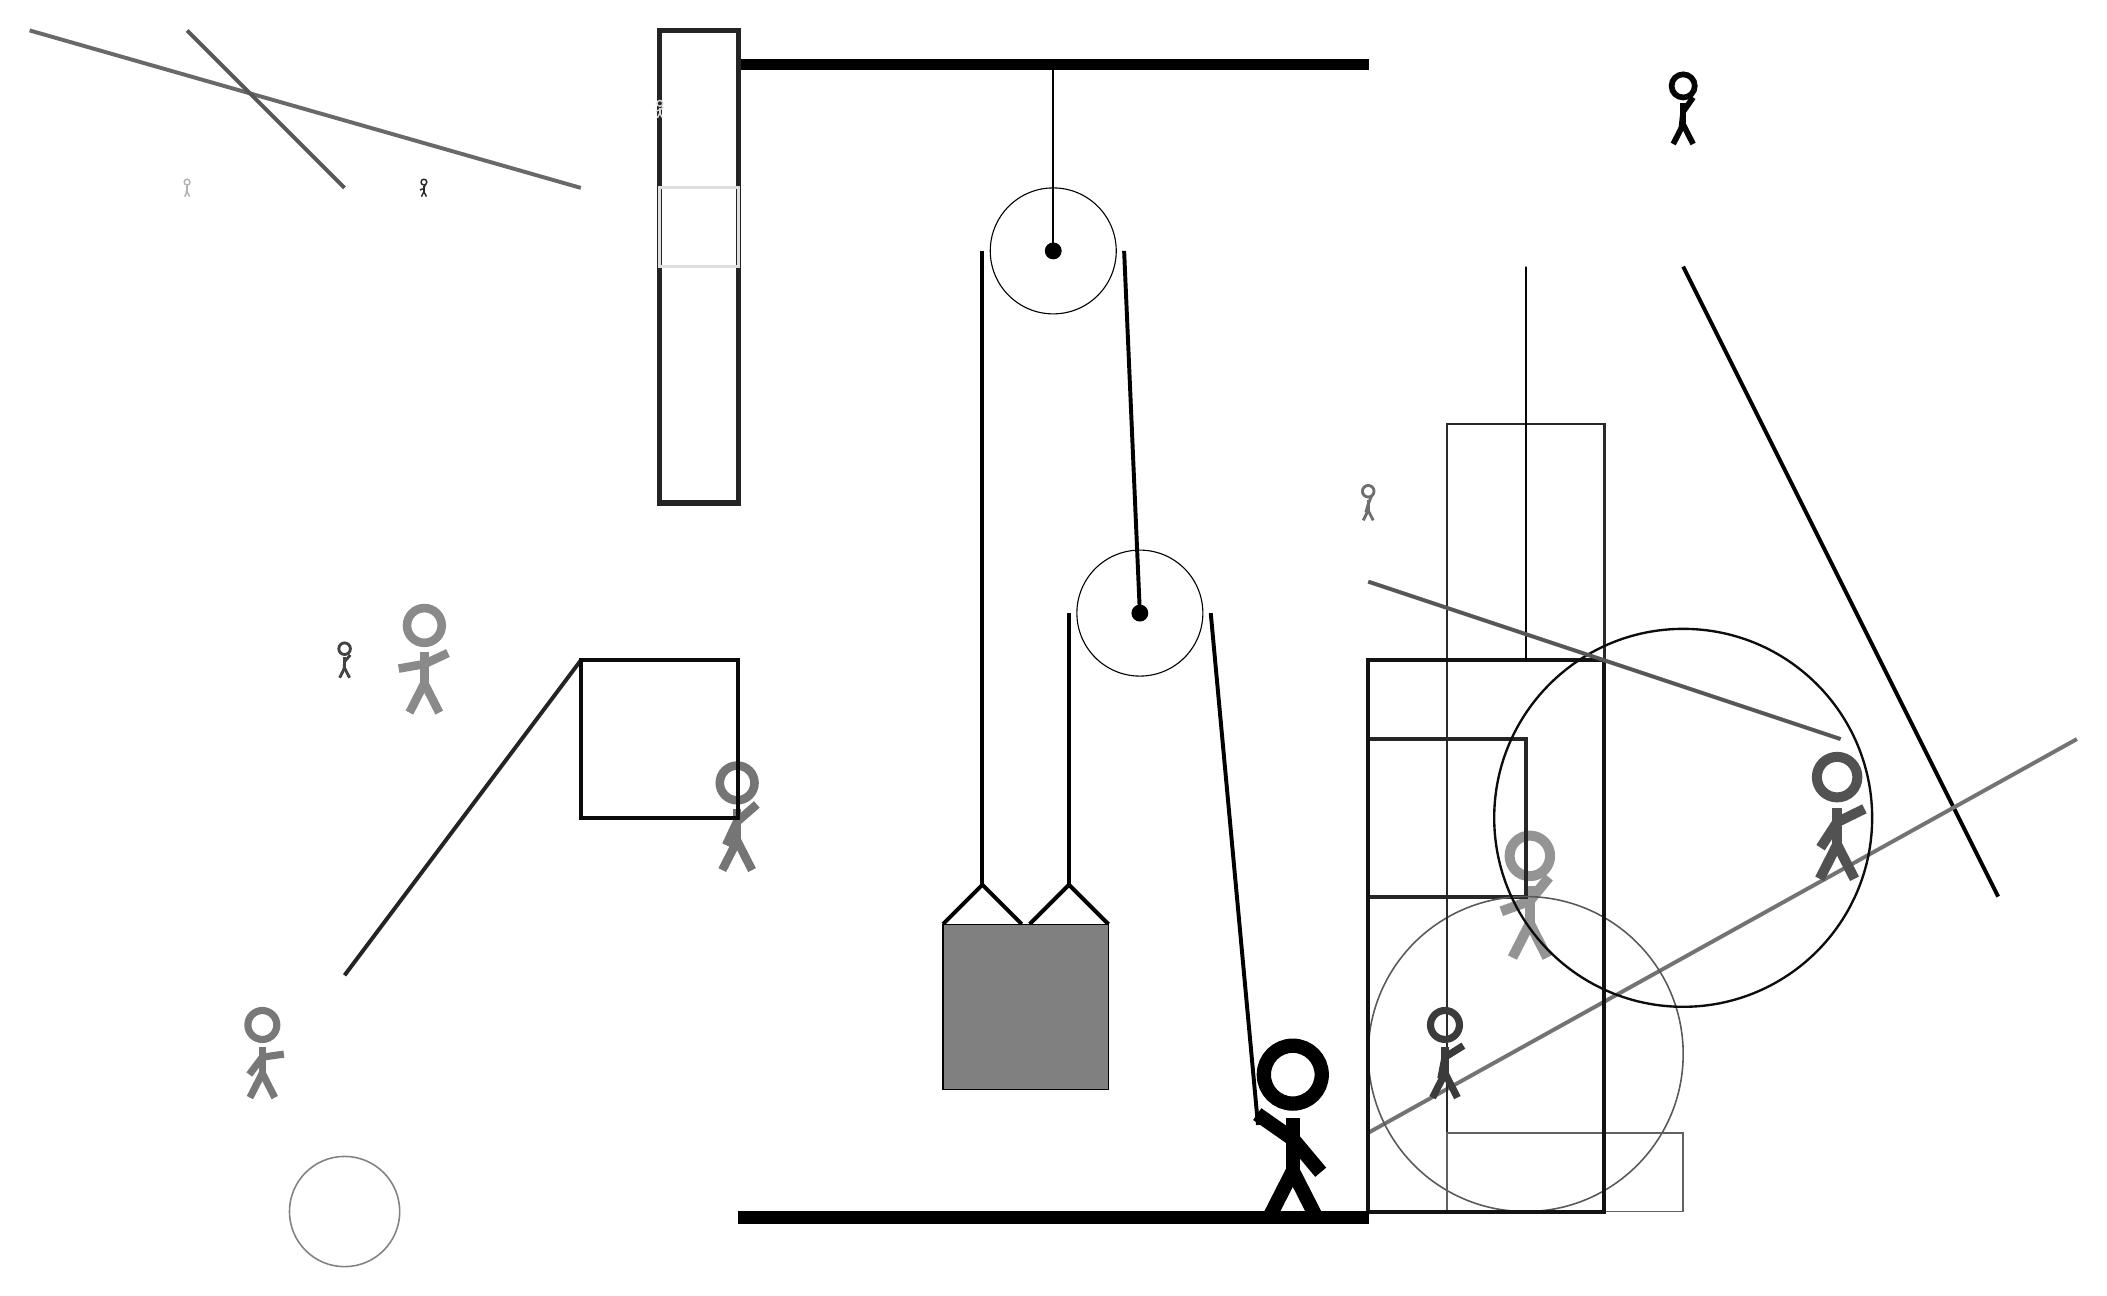
\begin{tikzpicture}
			%%%%% START %%%%%
			
			\draw[fill=black] (-2, 11.5) rectangle (6, 11.625);
			
			\draw (2, 9.2) circle (0.8);
			\draw[fill=black] (2, 9.2) circle (0.1);
			\draw[thick] (2, 9.2) -- (2, 11.5);
			
			\draw (3.1, 4.6) circle (0.8);
			\draw[fill=black] (3.1, 4.6) circle (0.1);
			
			\draw[line width=0.5mm, color=black!100](10, 9) -- (14, 1);
			
			\node[line width=0.5mm, color=black!42] at (8, 1) {\Strichmaxerl[7][20][51]};
			\draw[line width=0.5mm, color=black!85] (6, 3) rectangle (8, 1);
			\draw[line width=0.5mm, color=black!55](6, -2) -- (15, 3);
			\node[line width=0.7mm, color=black!98] at (10, 11) {\Strichmaxerl[4][84][55]};
			\node[line width=0.4mm, color=black!53] at (-8, -1) {\Strichmaxerl[5][53][8]};
			
			\draw [line width=0.2mm, color=black!65](8, -1) circle (2.0);
			
			\node[line width=0.3mm, color=black!46] at (-6, 4) {\Strichmaxerl[6][10][25]};
			\draw[line width=0.5mm, color=black!59](-4, 10) -- (-11, 12);
			\draw[line width=0.3mm, color=black!84] (7, 7) rectangle (9, -2);
			\node[line width=0.2mm, color=black!68] at (12, 2) {\Strichmaxerl[7][57][26]};
			\node[line width=0.3mm, color=black!84] at (-6, 10) {\Strichmaxerl[1][20][71]};
			\draw[line width=0.2mm, color=black!62] (7, -3) rectangle (10, -2);
			\node[line width=0.3mm, color=black!57] at (6, 6) {\Strichmaxerl[2][74][68]};
			\node[line width=0.2mm, color=black!54] at (-2, 2) {\Strichmaxerl[6][65][41]};
			\draw[line width=0.7mm, color=black!86] (-3, 6) rectangle (-2, 12);
			\node[line width=0.3mm, color=black!30] at (-9, 10) {\Strichmaxerl[1][75][85]};
			\draw[line width=0.5mm, color=black!86](-7, 0) -- (-4, 4);
			\draw[line width=0.5mm, color=black!93] (6, -3) rectangle (9, 4);
			\draw[line width=0.4mm, color=black!13] (-3, 9) rectangle (-2, 10);
			\draw [line width=0.3mm, color=black!95](10, 2) circle (2.4);
			
			\draw[line width=0.5mm, color=black!66](-7, 10) -- (-9, 12);
			\draw[line width=0.5mm, color=black!96] (-2, 4) rectangle (-4, 2);
			\draw[line width=0.3mm, color=black!98] (8, 9) rectangle (8, 4);
			\node[line width=0.5mm, color=black!77] at (7, -1) {\Strichmaxerl[5][79][32]};
			\draw[line width=0.5mm, color=black!66](6, 5) -- (12, 3);
			
			\node[line width=0.2mm, color=black!15] at (-3, 11) {\Strichmaxerl[1][18][37]};
			\draw [line width=0.2mm, color=black!49](-7, -3) circle (0.7);
			\node[line width=0.3mm, color=black!74] at (-7, 4) {\Strichmaxerl[2][86][49]};
			
			\draw[line width = 0.5mm]  (0.6, 0.65) -- (1.1, 1.15) -- (1.6, 0.65);
			\draw[line width = 0.5mm]  (1.7, 0.65) -- (2.2, 1.15) -- (2.7, 0.65);
			\draw[fill=black!50] (0.6, 0.65) rectangle (2.7, -1.45);
			
			\draw[line width = 0.5mm] (1.1, 9.2) -- (1.1, 1.15);
			\centerarc[line width = 0.5mm](2, 9.2)(0:180:0.9);
			\draw[line width = 0.5mm] (2.9, 9.2) -- (3.1, 4.6);
			\draw[line width = 0.5mm] (2.2, 4.6) -- (2.2, 1.15);
			\centerarc[line width = 0.5mm](3.1, 4.6)(0:180:0.9);
			\draw[line width = 0.5mm] (4.0, 4.6) -- (4.6, -1.9);
			
			\node at (5, -2) {\Strichmaxerl[10][-35][-50]};
			
			\draw[fill=black] (-2, -3) rectangle (6, -3.15);
			
			%%%%% END %%%%%
		\end{tikzpicture}
	\end{figure}	
\end{document}